\chapter{Komplexní čísla}


\begin{prolog}
:- ensure_loaded("../equations/formula").
:- ensure_loaded("../equations/truth_table").
:- ensure_loaded("../equations/draw_1d_function").

make_test_numbers([-1, 0, 0.5, 1, 2, 3, 1.5, complex(0, 1), complex(0, -1), complex(1, 1)]).
make_test_nonzero_complex_numbers([-1, 0.5, 1, 2, complex(0, 1), complex(0, -1), complex(1, 1), complex(0.2, -1.5)]).
make_test_real_numbers([-2, -1, 0, 1, 1.5, 2]).
make_test_nonnegative_real_numbers([0, 1, 1.5, 2]).
make_test_positive_real_numbers([1, 1.5, 2]).
make_test_real_nonzero_numbers([-2, -1, 1, 1.5, 2]).
make_test_complex_functions(Z, [Z + 2, Z - imag, (1 - imag) * Z, Z^2]).
make_test_real_binary_functions(X, Y, [X + Y, X * Y, X^2 * Y, Y^2 * X]).

make_test_analytic_functions(
	UX, UY, VX, VY,
	[
		[UX^2 - UY^2, 2 * VX * VY],
		[UX^3 - 3 * UX * UY^2, 3 * VX^2 * VY - VY^3]
	]
).

make_test_real_analytic_functions(   % Komplexni analyticke funkce, ktere jsou na realne osa realne
	UX, UY, VX, VY,
	[
		[UX^2 - UY^2, 2 * VX * VY],
		[UX^3 - 3 * UX * UY^2, 3 * VX^2 * VY - VY^3]
	]
).

make_test_harmonic_functions(
	UX, UY, [UX^2 - UY^2, 2 * UX * UY, UX^3 - 3 * UX * UY^2, 3 * UX^2 * UY - UY^3]
).

\end{prolog}

\section{Zavedení komplexních čísel}

V~sekci \ref{sec:realna_cisla} věnované reálným číslům jsme větou~\eqref{eq:sqrt_def} definovali odmocninu kladných čísel. Důvodem tohoto omezení je fakt, že v oboru reálných čísel neexistují sudé odmocniny ze záporných čísel. Například rovnice \(x^2 = -1\) nemá v~oboru reálných čísel řešení, neexistuje proto \(\sqrt{-1}\). Abychom mohli takovéto rovnice řešit, tak rovnicí~\eqref{eq:imag_def} zavedeme imaginární jednotku \(\imag\).

\begin{fact}
\begin{prolog}
?-	print_validated_formula(
		'imag_def',
		equal(imag^2, -1)
	).
\end{prolog}
\eeq{imag_def}
\end{fact}

Uvažujme dvě reálná čísla \(a\) a~\(b\), z~nichž alespoň jedno je nenulové. Chtějme nalézt takovou kombinaci těchto čísel, aby platilo:

\begin{prolog}
?-	make_test_numbers(Numbers),
	print_validated_formula(
		'complex_units_ortogonality',
		declare([variable(A, 'a', Numbers), variable(B, 'b', Numbers)],
			proof([
				equal(A * 1 + B * imag, 0)
			],
			[
				equal(A * 1, -B * imag),
				equal(A^2 * 1^2, B^2 * imag^2),
				equal(A^2, -B^2),
				equal(A^2 + B^2, 0)
			])
		)
	).
\end{prolog}
\eeq{complex_units_ortogonality}

Vidíme, že pro nenulová čísla tato rovnice nemůže být splněna. Reálná jednotka \(1\) a~imaginární jednotka \(\imag\) jsou proto navzájem ortogonální - jednu není možné vyjádřit pomocí druhé. Tyto jednotky si tedy můžeme představit jako vzájemně kolmé jednotkové osy ve dvojrozměrném prostoru. Každý bod v~tomto prostoru můžeme popsat jako lineární kombinaci těchto jednotek. Proto tuto lineární kombinaci \(a + b \cdot \imag\) nazveme komplexním číslem zapsaným v~algebraickém tvaru. Množinu všech komplexních čísel označíme \(\complex\).

\begin{fact}
\begin{prolog}
?-	make_test_numbers(Numbers),
	print_validated_formula(
		'complex_def',
		forall_in([A, B], ['a', 'b'], real_numbers, Numbers,
			in(A + B * imag, complex_numbers)
		)
	).
\end{prolog}
\eeq{complex_def}
\end{fact}

Vyjádřeme operace s~komplexními čísly. Využijeme přitom faktu, že se složkami můžeme provádět algebraické operace. Začněme součtem a~rozdílem komplexních čísel. Ten provádíme po složkách:

\begin{prolog}
?-	make_test_numbers(Numbers),
	print_validated_formula(
		'complex_add',
		declare([
			plus_minus(PM), variable(A, 'a', Numbers), variable(B, 'b', Numbers),
			variable(C, 'c', Numbers), variable(D, 'd', Numbers)
		],
			equal(
				plus_minus(par(A + B * imag), par(C + D * imag), PM),
				par(plus_minus(A, C, PM)) + par(plus_minus(B, D, PM)) * imag
			)
		)
	).
\end{prolog}
\eeq{complex_add}

Součin dvou komplexních čísel můžeme vyjádřit pomocí roznásobení výrazu:

\begin{prolog}
?-	make_test_numbers(Numbers),
	print_validated_formula(
		'complex_times',
		declare([variable(A, 'a', Numbers), variable(B, 'b', Numbers), variable(C, 'c', Numbers), variable(D, 'd', Numbers)],
			equal([
				(A + B * imag) * (C + D * imag),
				A * C + A * D * imag + B * C * imag + B * D * imag^2,
				linebreak,
				par(A * C - B * D) + (A * D  + B * C) * imag
			])
		)
	).
\end{prolog}
\eeq{complex_times}

Ke každému komplexnímu číslu \(a + b \cdot \imag\) můžeme zavést komplexně sdružené číslo \(a - b \cdot \imag\). Povšimněme si, že jejich součin daný vztahem~\eqref{eq:complex_multiply_by_conjugate} je reálný.

\begin{prolog}
?-	make_test_real_numbers(Numbers),
	print_validated_formula(
		'complex_multiply_by_conjugate',
		declare([variable(A, 'a', Numbers), variable(B, 'b', Numbers)],
			equal(
				(A + B * imag) * (A - B * imag),
				A^2 + B^2
			)
		)
	).
\end{prolog}
\eeq{complex_multiply_by_conjugate}

Toho můžeme využít pro vyjádření podílu dvou komplexních čísel:

\begin{prolog}
?-	make_test_real_numbers(Numbers),
	make_test_real_nonzero_numbers(NonzeroNumbers),
	print_validated_formula(
		'complex_fraction',
		declare([
			variable(A, 'a', Numbers), variable(B, 'b', Numbers),
			variable(C, 'c', NonzeroNumbers), variable(D, 'd', NonzeroNumbers)
		],
			equal([
				(A + B * imag) / (C + D * imag),
				((A + B * imag) * (C - D * imag)) / ((C + D * imag) * (C - D * imag)),
				linebreak,
				(A * C + B * D + B * C * imag - A * D * imag) / (C^2 + D^2),
				(A * C + B * D) / (C^2 + D^2) + (B * C - A * D) / (C^2 + D^2) * imag
			])
		)
	).
\end{prolog}
\eeq{complex_fraction}

Absolutní hodnota komplexního čísla \(x + Y \cdot \imag\) je dána výrazem \eqref{eq:complex_abs}. Jeho srovnáním se vztahem \eqref{eq:euklidovsky_prostor_metrika} dospějeme k~závěru, že komplexní rovina odpovídá dvojrozměrnému Euklidovskému prostoru.

\begin{prolog}
?-	make_test_real_numbers(Numbers),
	print_validated_formula(
		'complex_abs',
		declare([variable(X, 'x', Numbers), variable(Y, 'y', Numbers)],
			equal(abs(X + Y * imag), sqrt(X^2 + Y^2))
		)
	).
\end{prolog}
\eeq{complex_abs}

\section{Komplexní funkce, limita, derivace}

Mějme komplexní funkci komplexní proměnné \(z\):

\begin{equation}
w = \func{f}(z); z, w \in \complex
\end{equation}

Tuto funkci můžeme rozepsat na dvě reálné funkce dvou reálných proměnných:

\begin{equation}
\func{f}(x + y \cdot \imag) = \func{u}(x, y) + \func{v}(x, y) \cdot \imag
\end{equation}

Limitu komplexní funkce definujeme jako limitu funkce dvou parametrů. Znamená to tedy, že funkční hodnota se limitě musí blížit \uv{ze všech směrů}.

\begin{prolog}
?-	make_test_real_numbers(Numbers),
	make_test_complex_functions(P, Functions),
	print_validated_formula(
		'complex_lim',
		declare([variable(X0, 'x_0', Numbers), variable(Y0, 'y_0', Numbers), function(F, '\\func{f}', Functions)],
			equal(
				lim(Z, 'z', complex, X0 + Y0 * imag, apply(F, [P], [Z])),
				lim([X, Y], ['x', 'y'], [real, real], [X0, Y0], apply(F, [P], [X + Y * imag]))
			)
		)
	).
\end{prolog}
\eeq{complex_lim}

Derivaci komplexní funkce definujeme obdobně jako derivaci reálné funkce pomocí vztahu~\eqref{eq:complex_derivative}.

\begin{prolog}
?-	make_test_numbers(Numbers),
	make_test_complex_functions(P, Functions),
	print_validated_formula(
		"complex_derivative",
		declare([function(F, "\\func{f}", Functions), variable(Z, 'z', Numbers)],
			equal(
				derivative(Z, apply(F, [P], [Z])),
				lim(DZ, "\\mathrm{d}z", complex, 0, (apply(F, [P], [Z + DZ]) - apply(F, [P], [Z])) / DZ)
			)
		)
	).
\end{prolog}
\eeq{complex_derivative}

Zabývejme se otázkou, kdy tato derivace existuje. Nejdříve rozepišme definici derivace~\eqref{eq:complex_derivative} na podíl diferenciálů. Zavedeme tedy označení \(\func{f}(z + \mathrm{d}z) - \func{f}(z) = \mathrm{d}u + \mathrm{d}v \cdot \imag\) a~\(\mathrm{d}z = \mathrm{d}x + \mathrm{d}y \cdot \imag\):

\begin{prolog}
?-	make_test_real_numbers(Numbers),
	make_test_analytic_functions(UX, UY, VX, VY, Functions),
	print_validated_formula(
		"complex_derivative_conditions_1",
		declare([
			variable(X, "x", Numbers),
			variable(Y, "y", Numbers),
			function([U, V], ["\\func{u}", "\\func{v}"], Functions), 
			substitution(DU, "\\mathrm{d}u", apply(U, [UX, UY], [X + DX, Y + DY]) - apply(U, [UX, UY], [X, Y])),
			substitution(DV, "\\mathrm{d}v", apply(V, [VX, VY], [X + DX, Y + DY]) - apply(V, [VX, VY], [X, Y]))
		],
			equal([
				lim(
					[DX, DY], ["\\mathrm{d}x", "\\mathrm{d}y"], [real, real], [0, 0],
					(DU + DV * imag) / (DX + DY * imag)
				),
				lim([DX, DY], ["\\mathrm{d}x", "\\mathrm{d}y"], [real, real], [0, 0],
					((DU + DV * imag) / (DX + DY * imag)) * ((DX - DY * imag) / (DX - DY * imag))	
				),
				linebreak,
				lim(
					[DX, DY], ["\\mathrm{d}x", "\\mathrm{d}y"], [real, real], [0, 0],
					(DU * DX + DV * DY + (DV * DX - DU * DY) * imag) / (DX^2 + DY^2)
				)
			])
		)
	).
\end{prolog}
\eeq{complex_derivative_conditions_1}

Uvědomme si, že limita~\eqref{eq:complex_derivative_conditions_1} je definována pro dvojici proměnných~\(\mathrm{d}x\) a~\(\mathrm{d}y\). Proto můžeme zvolit \(\mathrm{d}x = 0\) a~limita se tím nezmění:

\begin{prolog}
?-	make_test_real_numbers(Numbers),
	make_test_analytic_functions(UX, UY, VX, VY, Functions),
	print_validated_formula(
		"complex_derivative_conditions_2",
		declare([
			function([U, V], ["\\func{u}", "\\func{v}"], Functions), 
			variable(X, "x", Numbers),
			variable(Y, "y", Numbers),
			substitution(DU, "\\mathrm{d}u", apply(U, [UX, UY], [X + DX, Y + DY]) - apply(U, [UX, UY], [X, Y])),
			substitution(DV, "\\mathrm{d}v", apply(V, [VX, VY], [X + DX, Y + DY]) - apply(V, [VX, VY], [X, Y]))
		],
			equal([
				lim(
					[DX, DY], ["\\mathrm{d}x", "\\mathrm{d}y"], [real, real], [0, 0],
					(DU + DV * imag) / (DX + DY * imag)
				),
				declare([substitution(DX, "\\mathrm{d}x", 0)],
					lim(
						DY, "\\mathrm{d}y", real, 0,
						(DV * DY - DU * DY * imag) / DY^2
					)
				),
				linebreak,
				declare([substitution(DX, "\\mathrm{d}x", 0)],
					lim(
						DY, "\\mathrm{d}y", real, 0,
						(DV - DU * imag) / DY
					)
				),
				derivative(Y, apply(V, [VX, VY], [X, Y])) - derivative(Y, apply(U, [UX, UY], [X, Y])) * imag
			])
		)
	).
\end{prolog}
\eeq{complex_derivative_conditions_2}

Obdobně můžeme zvolit \(\mathrm{d}y = 0\) a~získáme:

\begin{prolog}
?-	make_test_real_numbers(Numbers),
	make_test_analytic_functions(UX, UY, VX, VY, Functions),
	print_validated_formula(
		"complex_derivative_conditions_3",
		declare([
			function([U, V], ["\\func{u}", "\\func{v}"], Functions), 
			variable(X, "x", Numbers),
			variable(Y, "y", Numbers),
			substitution(DU, "\\mathrm{d}u", apply(U, [UX, UY], [X + DX, Y + DY]) - apply(U, [UX, UY], [X, Y])),
			substitution(DV, "\\mathrm{d}v", apply(V, [VX, VY], [X + DX, Y + DY]) - apply(V, [VX, VY], [X, Y]))
		],
			equal([
				lim(
					[DX, DY], ["\\mathrm{d}x", "\\mathrm{d}y"], [real, real], [0, 0],
					(DU + DV * imag) / (DX + DY * imag)
				),
				declare([substitution(DY, "\\mathrm{d}y", 0)],
					lim(
						DX, "\\mathrm{d}x", real, 0,
						(DU * DX + DV * DX * imag) / DX^2
					)
				),
				linebreak,
				declare([substitution(DY, "\\mathrm{d}y", 0)],
					lim(
						DX, "\\mathrm{d}x", real, 0,
						(DU + DV * imag) / DX
					)
				),
				derivative(X, apply(U, [UX, UY], [X, Y])) + derivative(X, apply(V, [VX, VY], [X, Y])) * imag
			])
		)
	).
\end{prolog}
\eeq{complex_derivative_conditions_3}

Srovnejme vztahy~\eqref{eq:complex_derivative_conditions_2} a~\eqref{eq:complex_derivative_conditions_3}. Dvě komplexní čísla jsou shodná, pokud mají stejnou reálnou i~imaginární složku. Proto má-li komplexní funkce derivaci, tak bude platit:

\begin{prolog}
?-	make_test_real_numbers(Numbers),
	make_test_analytic_functions(UX, UY, VX, VY, Functions),
	print_validated_formula(
		"complex_derivative_conditions_cauchy_riemann",
		declare([
			function([U, V], ["\\func{u}", "\\func{v}"], Functions),
			variable(X, "x", Numbers),
			variable(Y, "y", Numbers)
		],
			and(
				equal(derivative(X, apply(U, [UX, UY], [X, Y])), derivative(Y, apply(V, [VX, VY], [X, Y]))),
				equal(derivative(Y, apply(U, [UX, UY], [X, Y])), -derivative(X, apply(V, [VX, VY], [X, Y])))
			)
		)
	).
\end{prolog}
\eeq{complex_derivative_conditions_cauchy_riemann}

Podmínky~\eqref{eq:complex_derivative_conditions_cauchy_riemann} se nazývají Cauchyovy-Riemannovy podmínky. 
Má-li komplexní funkce derivaci v~každém bodě určité oblasti, pak říkáme, že je v~této oblasti analytická.

Zabývejme se otázkou, zda je splnění podmínek~\eqref{eq:complex_derivative_conditions_cauchy_riemann} postačující k~existenci derivace komplexní funkce. Ve vztazích~\eqref{eq:complex_derivative_conditions_2} a~\eqref{eq:complex_derivative_conditions_3} jsme položili \(\mathrm{d}x = 0\) respektive \(\mathrm{d}y = 0\), uvažovali jsme tedy pouze okolní body se stejnou reálnou respektive imaginární složkou. Potřebujeme ale ověřit, že všechny okolní body se blíží k~limitě~\eqref{eq:complex_derivative_conditions_1}. Pokračujme proto upravováním vztahu
~\eqref{eq:complex_derivative_conditions_1}

\begin{prolog}
?-	make_test_real_numbers(Numbers),
	make_test_analytic_functions(UX, UY, VX, VY, Functions),
	print_validated_formula(
		"complex_derivative_conditions_5",
		declare([
			function([U, V], ["\\func{u}", "\\func{v}"], Functions), 
			variable(X, "x", Numbers),
			variable(Y, "y", Numbers),
			substitution(DU, "\\mathrm{d}u", apply(U, [UX, UY], [X + DX, Y + DY]) - apply(U, [UX, UY], [X, Y])),
			substitution(DV, "\\mathrm{d}v", apply(V, [VX, VY], [X + DX, Y + DY]) - apply(V, [VX, VY], [X, Y]))
		],
			equal([
				lim(
					[DX, DY], ["\\mathrm{d}x", "\\mathrm{d}y"], [real, real], [0, 0],
					(DU * DX + DV * DY + (DV * DX - DU * DY) * imag) / (DX^2 + DY^2)
				),
				linebreak,
				lim(
					[DX, DY], ["\\mathrm{d}x", "\\mathrm{d}y"], [real, real], [0, 0],
					((DU / DX) * DX^2 + (DV / DY) * DY^2 + ((DV / DX) * DX^2 - (DU / DY) * DY^2) * imag) / (DX^2 + DY^2)
				),
				linebreak,
				lim(
					[DX, DY], ["\\mathrm{d}x", "\\mathrm{d}y"], [real, real], [0, 0],
					(derivative(X, apply(U, [UX, UY], [X, Y])) * DX^2 + derivative(Y, apply(V, [VX, VY], [X, Y])) * DY^2 + (derivative(X, apply(V, [VX, VY], [X, Y])) * DX^2 - derivative(Y, apply(U, [UX, UY], [X, Y])) * DY^2) * imag) / (DX^2 + DY^2)
				),
				linebreak,
				lim(
					[DX, DY], ["\\mathrm{d}x", "\\mathrm{d}y"], [real, real], [0, 0],
					(derivative(X, apply(U, [UX, UY], [X, Y])) * DX^2 + derivative(X, apply(U, [UX, UY], [X, Y])) * DY^2 + (derivative(X, apply(V, [VX, VY], [X, Y])) * DX^2 + derivative(X, apply(V, [VX, VY], [X, Y])) * DY^2) * imag) / (DX^2 + DY^2)
				),
				linebreak,
				lim(
					[DX, DY], ["\\mathrm{d}x", "\\mathrm{d}y"], [real, real], [0, 0],
					(derivative(X, apply(U, [UX, UY], [X, Y])) * (DX^2 + DY^2) + (derivative(X, apply(V, [VX, VY], [X, Y])) * (DX^2 + DY^2)) * imag) / (DX^2 + DY^2)
				),
				linebreak,
				lim(
					[DX, DY], ["\\mathrm{d}x", "\\mathrm{d}y"], [real, real], [0, 0],
					derivative(X, apply(U, [UX, UY], [X, Y])) + derivative(X, apply(V, [VX, VY], [X, Y])) * imag
				)
			])
		)
	).
\end{prolog}
\eeq{complex_derivative_conditions_5}

Vidíme, že podmínky~\eqref{eq:complex_derivative_conditions_cauchy_riemann} jsou podmínky nutné i~postačující.

\begin{prolog}
?-	make_test_real_numbers(Numbers),
	make_test_analytic_functions(UX, UY, VX, VY, Functions),
	print_validated_multiformula(
		[
			function([U, V], ["\\func{u}", "\\func{v}"], Functions), 
			variable(X, "x", Numbers),
			variable(Y, "y", Numbers),
			substitution(DU, "\\func{u'}", derivative(DUX, apply(U, [UX, UY], [DUX, DUY]))),
			substitution(DV, "\\func{v'}", derivative(DVX, apply(V, [VX, VY], [DVX, DVY])))
		],
		[
			formula(
				"complex_derivative_analytic_1",
				equal([
					apply(DU, [DUX, DUY], [X, Y]),
					derivative(X, apply(U, [UX, UY], [X, Y])),
					derivative(Y, apply(V, [VX, VY], [X, Y]))
				])
			),
			formula(
				"complex_derivative_analytic_2",
				equal([
					apply(DV, [DVX, DVY], [X, Y]),
					derivative(X, apply(V, [VX, VY], [X, Y])),
					-derivative(Y, apply(U, [UX, UY], [X, Y]))
				])
			),
			formula(
				"complex_derivative_analytic_3",
				equal([
					derivative(X, apply(DU, [DUX, DUY], [X, Y])),
					derivative(X * Y, apply(V, [VX, VY], [X, Y])),
					derivative(Y, apply(DV, [DVX, DVY], [X, Y]))	
				])
			),
			formula(
				"complex_derivative_analytic_4",
				equal([
					derivative(Y, apply(DU, [DUX, DUY], [X, Y])),
					derivative(X * Y, apply(U, [UX, UY], [X, Y])),
					-derivative(X, apply(DV, [DVX, DVY], [X, Y]))	
				])
			)
		]
	).
\end{prolog}

Uvažujme dále. Mějme analytickou funkci \(\func{u}(x, y) + \func{v}(x, y) \cdot \imag\). Její derivaci označme \(\func{u'}(x, y) + \func{v'}(x, y) \cdot \imag\). Platí tedy
\eeq{complex_derivative_analytic_1}
\eeq{complex_derivative_analytic_2}

Vidíme, že platí
\eeq{complex_derivative_analytic_3}
\eeq{complex_derivative_analytic_4}
a~derivace analytické funkce je tedy opět analytická funkce.

\section{Analytická funkce jako řešení Laplaceovy rovnice}
\label{sec:complex_analytical_laplace}

Vyjděme z~Cauchyových-Riemannových podmínkek.

\begin{prolog}
?-	make_test_real_numbers(Numbers),
	make_test_analytic_functions(UX, UY, VX, VY, Functions),
	print_validated_multiformula(
		[
			function([U, V], ["\\func{u}", "\\func{v}"], Functions),
			variable(X, "x", Numbers),
			variable(Y, "y", Numbers)
		],
		[
			% Cauchyovy-Riemannovy podminky 
			formula(
				"analytic_function_laplace_cr1",
				equal(derivative(X, apply(U, [UX, UY], [X, Y])), derivative(Y, apply(V, [VX, VY], [X, Y])))
			),
			formula(
				"analytic_function_laplace_cr2",
				equal(derivative(Y, apply(U, [UX, UY], [X, Y])), -derivative(X, apply(V, [VX, VY], [X, Y])))
			),
			
			% Laplace U
			formula(
				"analytic_function_laplace_u1",
				equal(derivative(X^2, apply(U, [UX, UY], [X, Y])), derivative(X * Y, apply(V, [VX, VY], [X, Y])))
			),
			formula(
				"analytic_function_laplace_u2",
				equal(derivative(Y^2, apply(U, [UX, UY], [X, Y])), -derivative(X * Y, apply(V, [VX, VY], [X, Y])))
			),
			formula(
				"analytic_function_laplace_u_sum",
				equal(derivative(X^2, apply(U, [UX, UY], [X, Y])) + derivative(Y^2, apply(U, [UX, UY], [X, Y])), 0)
			),
			
			% Laplace V
			formula(
				"analytic_function_laplace_v1",
				equal(derivative(X * Y, apply(U, [UX, UY], [X, Y])), derivative(Y^2, apply(V, [VX, VY], [X, Y])))
			),
			formula(
				"analytic_function_laplace_v2",
				equal(derivative(X * Y, apply(U, [UX, UY], [X, Y])), -derivative(X^2, apply(V, [VX, VY], [X, Y])))
			),
			formula(
				"analytic_function_laplace_v_sum",
				equal(derivative(X^2, apply(V, [VX, VY], [X, Y])) + derivative(Y^2, apply(V, [VX, VY], [X, Y])), 0)
			)
		]
	).
\end{prolog}

\eeq{analytic_function_laplace_cr1}
\eeq{analytic_function_laplace_cr2}

Zderivujme rovnici~\eqref{eq:analytic_function_laplace_cr1} podle \(x\) a~rovnici~\eqref{eq:analytic_function_laplace_cr2} podle \(y\). Získáme:

\eeq{analytic_function_laplace_u1}
\eeq{analytic_function_laplace_u2}

Jejich sečtením získáme rovnici

\eeq{analytic_function_laplace_u_sum}

Zderivujme rovnici~\eqref{eq:analytic_function_laplace_cr1} podle \(y\) a~rovnici~\eqref{eq:analytic_function_laplace_cr2} podle \(x\). Získáme:

\eeq{analytic_function_laplace_v1}
\eeq{analytic_function_laplace_v2}

Jejich sloučením získáme rovnici

\eeq{analytic_function_laplace_v_sum}

Vidíme tedy, že funkce \(\func{u}\) i~\(\func{v}\) jsou řešením Laplaceovy rovnice v~rovině. Reálná i~imaginární složka analytické funkce je proto řešením Laplaceovy rovnice v~rovině.

\section{Rozšíření reálných funkcí do komplexního oboru}

Mějme reálnou funkci reálné proměnné \(\func{f_r}(x)\) . Uvažujme, že chceme rozšířit její definiční obor na komplexní čísla a~to tak, aby výsledná funkce byla analytická. Předpokládejme, že existují dvě různé rozšířené komplexní funkce komplexních proměnných, označme je \(\func{f_1}(z)\) a~\(\func{f_2}(z)\). Jejich rozdíl - také analytickou funkci - označme \(\func{\Delta f}(z) = \func{f_2}(z) - \func{f_1}(z) = u(x, y) + v(x, y) \cdot \imag\). Víme tedy, že \(u(x, 0) = 0\), protože na reálné ose si musejí být obě funkce \(\func{f_1}\) a~\(\func{f_2}\) sobě rovny. Dále víme, že \(v(x, 0) = 0\), protože na reálné ose nemohou mít funkce \(\func{f_1}\) a~\(\func{f_2}\) imaginární složky. Platí tedy \(\frac{\partial v}{\partial x}(x, 0) = -\frac{\partial u}{\partial y}(x, 0) = 0\), stejně jako \(\frac{\partial u}{\partial x}(x, 0) = \frac{\partial v}{\partial y}(x, 0) = 0\). Shrňme si tedy poznatky, které víme o~funkci \(u\):

\begin{equation}
\begin{split}
u(x, 0) = 0 \\
\frac{\partial u}{\partial y}(x, 0) = 0 \\
\frac{\partial^2 u}{\partial x^2} + \frac{\partial^2 u}{\partial y^2} = 0
\end{split}
\end{equation}

Poslední rovnice je Laplaceova rovnice, jejíž platnost pro komplexní čísla jsme odvodili v~sekci \ref{sec:complex_analytical_laplace}. Laplaceova rovnice je invariantní vůčí posunutí (je ve všech bodech stejná). Stejně tak počáteční podmínky jsou pro všechny souřadnice \(x\) stejné. Můžeme tedy předpokládat, že řešení bude ve tvaru \(u(x, y) = u(y)\). Rovnice se nám tak zjednoduší na obyčejnou diferenciální rovnici druhého řádu

\begin{equation}
\begin{split}
u(0) = 0 \\
\frac{\partial u}{\partial y}(0) = 0 \\
\frac{\partial^2 u}{\partial y^2} = 0
\end{split}
\end{equation}

s~jediným řešením \(u(y) = u(x, y) = 0\). Obdobně můžeme sestavit rovnici

\begin{equation}
\begin{split}
v(x, 0) = 0 \\
\frac{\partial v}{\partial y}(x, 0) = 0 \\
\frac{\partial^2 v}{\partial x^2} + \frac{\partial^2 v}{\partial y^2} = 0
\end{split}
\end{equation}

s~jediným řešením \(v(x, y) = 0\). Víme tedy, že platí \(\func{\Delta f}(z) = 0\), funkce \(\func{f_1}(z)\) a~\(\func{f_2}(z)\) tedy musejí být shodné. Z toho plyne fakt:

\begin{fact}
Rozšíříme-li definiční obor funkce \(y = \func{f_r}(x); x \in \real, y \in \real\) na komplexní funkci \(w = \func{f_c}(z); z \in \complex, w \in \complex\) tak, aby komplexní funkce byla analytická, pak je tato funkce \(\func{f_c}\) plně určena funkcí \(\func{f_r}\).
\end{fact}

Víme, že derivací analytické funkce získáme opět analytickou funkci. Dále víme, že rozšíření reálné funkce na komplexní analytickou funkci je jednoznačně určeno onou reálnou funkcí. Z~toho plyne závěr:

\begin{fact}
Rozšíříme-li reálné funkce na komplexní analytické funkce, pak se tyto komplexní analytické funkce derivují stejně jako reálné.
\end{fact}

Například následující komplexní funkci můžeme zderivovat 

\begin{prolog}
?-	make_test_numbers(Numbers),
	print_validated_formula(
		"complex_real_analytic_1",
		declare(	[variable(Z, "z", Numbers)],
			equal(
				derivative(Z, Z^2 * e^(2*Z + 1)),
				2 * Z * e^(2*Z + 1) + 2 * Z^2 * e^(2*Z + 1)
			)
		)
	).
\end{prolog}
\eeq{complex_real_analytic_1}

protože odpovídající reálná funkce má derivaci:

\begin{prolog}
?-	make_test_real_numbers(Numbers),
	print_validated_formula(
		"complex_real_analytic_2",
		declare(	[variable(X, "x", Numbers)],
			equal(
				derivative(X, X^2 * e^(2*X + 1)),
				2 * X * e^(2*X + 1) + 2 * X^2 * e^(2*X + 1)
			)
		)
	).
\end{prolog}
\eeq{complex_real_analytic_2}

\section{Funkce sinus a~kosinus, Eulerův vzorec}

Úhel sevřený dvěma polopřímkami se společným bodem v~obloukové míře je udáván délkou oblouku, které tyto dvě polopřímky vytknou na jednotkové kruřnici. Udává se v~radiánech. Plný úhel má proto velikost \(2 \pi \ \rad\), přímý úhel \(\pi \ \rad\) a~pravý úhel \(\frac{\pi}{2} \ \rad\).

\begin{figure}[ht]
\begin{center}
\begin{tikzpicture}

\pgfmathsetmacro{\ang}{45}
\pgfmathsetmacro{\r}{4}
\pgfmathsetmacro{\p}{5}
\pgfmathsetmacro{\x}{cos(\ang)}
\pgfmathsetmacro{\y}{sin(\ang)}

\draw (0, 0) -- (\r, 0);
\draw[dashed] (\r, 0) -- (\p, 0);
\draw (\r / 2, 0) node[anchor=north]{1};

\draw (0, 0) -- (\r * \x, \r * \y);
\draw[dashed] (\r * \x, \r * \y) -- (\p * \x, \p * \y);
\draw (\r / 2 * \x, \r / 2 * \y) node[anchor=south east]{1};

\draw[->] (\r, 0) arc(0:\ang:\r);
\draw (\r * 0.92388, \r * 0.38268) node[anchor=west]{\(\alpha\)};
\end{tikzpicture}
\caption{Oblouková míra úhlu}
\label{img:rad_def}
\end{center}
\end{figure}

Mějme kartézský souřadný systém v~rovině, jak je zobrazeno na obrázku~\ref{img:sin_cos_def}. Dále mějme úsečku s~počátečním bodem v~počátku souřadného systému délkou 1. Tato úsečka bude svírat s~osou \(x\) orientovaný úhel \(\alpha\). Potom koncový bod této úsečky bude mít souřadnice \([x, y] = [\cos \alpha, \sin \alpha]\). Pokud by úsečka měla obecně délku \(r\), pak bz souřadnice bodu byly proporcionálně větší, tedy \([x, y] = [r \cdot \cos \alpha, r \cdot \sin \alpha]\). Funkce jsou zobrazeny na obrázcích~\ref{img:sin_function} a~\ref{img:cos_function}.

\begin{prolog}
?-	draw_1d_function(
		'sin_function',
		X,
		'x',
		sin(X),
		-2*pi, +2*pi
	).				
\end{prolog}
\eimg{sin_function}{Graf funkce sinus}

\begin{prolog}
?-	draw_1d_function(
		'cos_function',
		X,
		'x',
		cos(X),
		-2*pi, +2*pi
	).				
\end{prolog}
\eimg{cos_function}{Graf funkce kosinus}

\begin{figure}[ht]
\begin{center}
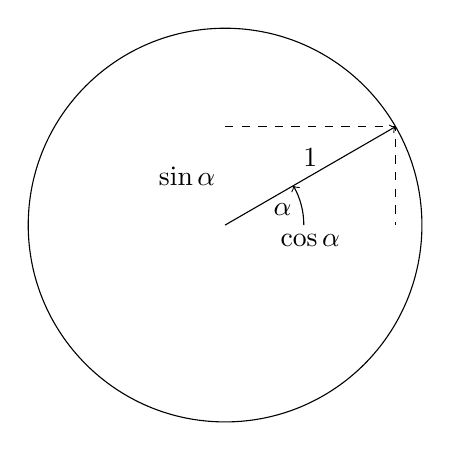
\begin{tikzpicture}

\pgfmathsetmacro{\r}{2.5}
\pgfmathsetmacro{\axr}{1.2 * \r}

\pgfmathsetmacro{\ang}{30}
\pgfmathsetmacro{\x}{cos(\ang)}
\pgfmathsetmacro{\y}{sin(\ang)}

\drawaxesxy{0}{0}{-\axr}{-\axr}{+\axr}{+\axr};
\draw (0, 0) circle[radius=\r];

\draw[->] (0, 0) -- (\r * \x, \r * \y);

\draw[dashed] (0, \r * \y) -- (\r * \x, \r * \y) -- (\r * \x, 0);

\draw (\r * \x / 2, 0) node[anchor=north]{\(\cos \alpha\)};
\draw (0, \r * \y / 2) node[anchor=east]{\(\sin \alpha\)};
\draw (\r / 2 * \x, \r / 2 * \y) node[anchor=south]{1};

\draw[->] (1, 0) arc(0:\ang:1);
\draw (0.96593, 0.2) node[anchor=east]{\(\alpha\)};

\drawrightangle{\r * \x}{0}{0.3}{90};
\drawrightangle{0}{\r * \y}{0.3}{270};
\end{tikzpicture}
\caption{Definice sinu a~kosinu}
\label{img:sin_cos_def}
\end{center}
\end{figure}


Odvoďme nyní derivaci funkcí sinus a~kosinus. Mějme opět jednotkovou úsečku OA s~jedním koncem v~počátku soustavy souřadnic, jak je zobrazeno na obrázku \eqref{img:sin_cos_derivative}. Tato úsečka svírá s~osou \(x\) orientovaný úhel \(\alpha\) a~její koncový bod A má tedy souřadnice \([\cos \alpha, \sin \alpha]\). Mějme další úsečku OB, která svírá s~osou \(x\) úhel o~\(\mathrm{d}\alpha\) větší. Její koncový bod B má tedy souřadnice \([\cos (\alpha + \mathrm{d}\alpha), \sin (\alpha + \mathrm{d}\alpha)]\). Oblouk kružnice mezi body A a~B má podle definice obloukové míry délku~\(\mathrm{d}\alpha\). Pro \(\mathrm{d}\alpha \to 0\) tento oblouk přechází v~úsečku. Proto pro \(\mathrm{d}\alpha\) je délka sečny \(|AB| = \mathrm{d}\alpha\). Dále si uvědomme, že pro \(\mathrm{d}\alpha \to 0\) sečna AB přechází v~tečnu a~je proto kolmá na úsečku OA, která je poloměrem kružnice. Díky tomu úsečka BA svírá s~(opačnou) osou y úhel \(\alpha\). Proto v~bodě B můžeme zavést lokální souřadný systém s~osou x mířící směrem dolů a~odvodit:

\begin{prolog}
?-	make_test_real_numbers(Numbers),
	print_validated_formula(
		"sin_derivative_proof",
		declare([
			variable(A, "\\alpha", Numbers) 
		],
			proof([],
			[
				declare(
					[substitution(DA, "\\mathrm{d}\\alpha", 1e-8)],
					equal(sin(A + DA) - sin(A), DA * cos(A))
				),
				equal(lim(DA, "\\mathrm{d}\\alpha", real, 0, (sin(A + DA) - sin(A)) / DA), cos(A)),
				equal(derivative(A, sin(A)), cos(A))
			])
		)
	).
\end{prolog}
\eeq{sin_derivative_proof}

\begin{prolog}
?-	make_test_real_numbers(Numbers),
	print_validated_formula(
		"cos_derivative_proof",
		declare([
			variable(A, "\\alpha", Numbers) 
		],
			proof([],
			[
				declare(
					[substitution(DA, "\\mathrm{d}\\alpha", 1e-8)],
					equal(cos(A + DA) - cos(A), -(DA * sin(A)))
				),
				equal(lim(DA, "\\mathrm{d}\\alpha", real, 0, (cos(A + DA) - cos(A)) / DA), -sin(A)),
				equal(derivative(A, cos(A)), -sin(A))
			])
		)
	).
\end{prolog}
\eeq{cos_derivative_proof}

\begin{figure}[ht]
\begin{center}
\begin{tikzpicture}
\pgfmathsetmacro{\r}{10}
\pgfmathsetmacro{\axr}{1.2 * \r}

\pgfmathsetmacro{\ang}{30}
\pgfmathsetmacro{\x}{cos(\ang)}
\pgfmathsetmacro{\y}{sin(\ang)}

\pgfmathsetmacro{\angb}{40}
\pgfmathsetmacro{\xb}{cos(\angb)}
\pgfmathsetmacro{\yb}{sin(\angb)}

\pgfmathsetmacro{\angd}{atan((\xb - \x) / (\y - \yb))}

\draw (0, 0) node[anchor=north east]{O};
\draw[->] (0, 0) -- (\r * \x, \r * \y) node[anchor=south west]{A};
\draw[dashed] (0, \r * \y) -- (\r * \x, \r * \y) -- (\r * \x, 0);

\draw (\r * \x, 0) node[anchor=north]{\(\cos \alpha\)};
\draw (\r * \xb, 0) node[anchor=north east]{\(\cos(\alpha + \mathrm{d}\alpha)\)};

\draw (0, \r * \y) node[anchor=east]{\(\sin \alpha\)};
\draw (0, \r * \yb) node[anchor=east]{\(\sin(\alpha + \mathrm{d}\alpha)\)};

\draw (\r / 2 * \x, \r / 2 * \y) node[anchor=north]{1};

\draw[->] (0, 0) -- (\r * \xb, \r * \yb) node[anchor=south west]{B};

\draw (\r * \xb, \r * \yb) -- (\r * \x, \r * \y);
\draw[dashed] (0, \r * \yb) -- (\r * \xb, \r * \yb) -- (\r * \xb, 0);

\draw(\r, 0) arc(-0:90:\r);
\drawaxesxy{0}{0}{-0.5}{-0.5}{+\axr}{+\axr};

\draw[->] (1, 0) arc(0:\ang:1);
\draw (0.96593, 0.2) node[anchor=east]{\(\alpha\)};
\draw (\r * \xb, \r * \yb - 0.5) node[anchor=north west]{\(\alpha\)};

\drawsmallangle{0}{0}{1.5}{\ang}{\angb}{\(\mathrm{d}\alpha\)};
\drawrightangle{\r * \xb}{\r * \y}{0.3}{0};

\draw (\r * \x / 2 + \r * \xb / 2, \r * \y / 2 + \r * \yb / 2) node[anchor=west]{\(\mathrm{d}\alpha\)};

\draw[->] (\r * \xb - 1.8, 2) -- (\r * \xb, 2);
\draw (\r * \xb, 2) -- (\r * \x, 2);
\draw[<-] (\r * \x, 2) -- (\r * \x + 0.3, 2);
\draw (\r * \xb - 0.2, 2) node[anchor=south east]{\(\mathrm{d}\alpha \cdot \cos \alpha\)};

\draw[<->] (2, \r * \yb) -- (2, \r * \y);
\draw (2, \r * \yb / 2 + \r * \y / 2) node[anchor=west]{\(\mathrm{d}\alpha \cdot \sin \alpha\)};

\draw[->] (\r * \xb, \r * \yb - 1) arc(270:270+\angd:1);

\drawrightangle{\r * \x}{0}{0.3}{90};
\drawrightangle{\r * \xb}{0}{0.3}{90};
\drawrightangle{0}{\r * \y}{0.3}{270};
\drawrightangle{0}{\r * \yb}{0.3}{270};
\end{tikzpicture}
\caption{Derivace funkcí sinus a~kosinus}
\label{img:sin_cos_derivative}
\end{center}
\end{figure}

Zabývejme se dále exponenciální funkcí \(e^{x \cdot \imag}\). Její derivace je

\begin{prolog}
?-	make_test_real_numbers(Numbers),
	print_validated_formula(
		"exp_sin_cos_proof_1",
		declare([
			variable(X, "x", Numbers),
			substitution(U, "\\mathrm{u}", cos(UX)),
			substitution(V, "\\mathrm{v}", sin(VX)) 
		],
			proof([],
			[
				equal(e^(X * imag), apply(U, [UX], [X]) + apply(V, [VX], [X]) * imag),
				equal(derivative(X, e^(X * imag)), e^(X * imag) * imag),
				equal(
					derivative(X, apply(U, [UX], [X]) + apply(V, [VX], [X]) * imag),
					(apply(U, [UX], [X]) + apply(V, [VX], [X]) * imag) * imag
				),
				equal(
					derivative(X, apply(U, [UX], [X])) + derivative(X, apply(V, [VX], [X])) * imag,
					-apply(V, [VX], [X]) + apply(U, [UX], [X]) * imag
				),
				and(
					equal(derivative(X, apply(U, [UX], [X])), -apply(V, [VX], [X])),
					equal(derivative(X, apply(V, [VX], [X])), apply(U, [UX], [X]))
				)
			])
		)
	).
\end{prolog}
\eeq{exp_sin_cos_proof_1}

Obdobně můžeme odvodit hodnoty funkcí pro \(x = 0\):


\begin{prolog}
?-	print_validated_formula(
		"exp_sin_cos_proof_2",
		declare([
			substitution(U, "\\mathrm{u}", cos(UX)),
			substitution(V, "\\mathrm{v}", sin(VX)) 
		],
			proof([],
			[
				equal(e^(0 * imag), 1),
				equal(
					apply(U, [UX], [0]) + apply(V, [VX], [0]) * imag,
					1 + 0 * imag
				),
				and(
					equal(apply(U, [UX], [0]), 1),
					equal(apply(V, [VX], [0]), 0)
				)
			])
		)
	).
\end{prolog}
\eeq{exp_sin_cos_proof_2}

Už víme, že platí

\begin{prolog}
?-	make_test_real_numbers(Numbers),
	print_validated_formula(
		"exp_sin_cos_proof_3",
		declare([
			variable(X, "x", Numbers)
		],
			and(
				equal(derivative(X, cos(X)), -sin(X)),
				equal(derivative(X, sin(X)), cos(X))
			)
		)
	).
\end{prolog}
\eeq{exp_sin_cos_proof_3}


a~z~obrázku~\ref{img:sin_cos_def} jsou také vidět hodnoty: 

\begin{prolog}
?-	print_validated_formula(
		"exp_sin_cos_proof_4",
			and(
				equal(cos(0), 1),
				equal(sin(0), 0)
		)
	).
\end{prolog}
\eeq{exp_sin_cos_proof_4}

Jak vztahy~\eqref{eq:exp_sin_cos_proof_1} a~\eqref{eq:exp_sin_cos_proof_2}, tak i~vztahy~\eqref{eq:exp_sin_cos_proof_3} a~\eqref{eq:exp_sin_cos_proof_4} představují sosutavy dvou obyčejných diferenciálních rovnic prvního řádu.
Protože hodnoty v~počátku i~průběh prvních derivací jsou si rovny, tak platí

\begin{prolog}
?-	make_test_real_numbers(Numbers),
	print_validated_formula(
		"exp_sin_cos_proof_result",
		declare([
			variable(X, "x", Numbers),
			substitution(U, "\\mathrm{u}", cos(UX)),
			substitution(V, "\\mathrm{v}", sin(VX)) 
		],
			proof([],
			[
				and(
					equal(apply(U, [UX], [X]), cos(X)),
					equal(apply(V, [VX], [X]), sin(X))
				),
				equal(e^(X * imag), cos(X) + imag * sin(X))
			])
		)
	).
\end{prolog}
\eeq{exp_sin_cos_proof_result}

To je známý Eulerův vzorec udávající vztah mezi exponenciální funkcí komplexního čísla a~goniometrickými funkcemi.

Eulerův vzorec můžeme využít pro odvození některých goniometrických identit. Například odvodíme vztah pro sinus a~kosinus součtu úhlů:

\begin{prolog}
?-	make_test_real_numbers(Numbers),
	print_validated_formula(
		"cos_sin_a_plus_b",
		declare([
			variable(A, "\\alpha", Numbers),
			variable(B, "\\beta", Numbers)
		],
			equal([
				cos(A + B) + imag * sin(A + B),
				e^(imag * (A + B)),
				e^(imag * A) * e^(imag * B),
				linebreak,
				(cos(A) + imag * sin(A)) * (cos(B) + imag * sin(B)),
				linebreak,
				cos(A) * cos(B) - sin(A) * sin(B) + imag * (cos(A) * sin(B) + sin(A) * cos(B))
			])
		)
	).
\end{prolog}
\eeq{cos_sin_a_plus_b}

Dvě komplexní čísla jsou shodná, pokud mají stejnou reálnou i~imaginární složku. Proto

\begin{prolog}
?-	make_test_real_numbers(Numbers),
	print_validated_formula(
		"cos_a_plus_b",
		declare([
			variable(A, "\\alpha", Numbers),
			variable(B, "\\beta", Numbers)
		],
			equal(cos(A + B), cos(A) * cos(B) - sin(A) * sin(B))
		)
	).
\end{prolog}
\eeq{cos_a_plus_b}
%%%%%%%%%%%%%%%%%%%%
\begin{prolog}
?-	make_test_real_numbers(Numbers),
	print_validated_formula(
		"sin_a_plus_b",
		declare([
			variable(A, "\\alpha", Numbers),
			variable(B, "\\beta", Numbers)
		],
			equal(sin(A + B), cos(A) * sin(B) + sin(A) * cos(B))
		)
	).
\end{prolog}
\eeq{sin_a_plus_b}

Substitucí \(\beta \leftarrow -\beta\) a~využitím faktu, že sinus je lichá funkce a~kosinus sudá, získáme:

\begin{prolog}
?-	make_test_real_numbers(Numbers),
	print_validated_formula(
		"cos_a_minus_b",
		declare([
			variable(A, "\\alpha", Numbers),
			variable(B, "\\beta", Numbers)
		],
			equal(cos(A - B), cos(A) * cos(B) + sin(A) * sin(B))
		)
	).
\end{prolog}
\eeq{cos_a_minus_b}
%%%%%%%%%%%%%%%%%%%%
\begin{prolog}
?-	make_test_real_numbers(Numbers),
	print_validated_formula(
		"sin_a_minus_b",
		declare([
			variable(A, "\\alpha", Numbers),
			variable(B, "\\beta", Numbers)
		],
			equal(sin(A - B), sin(A) * cos(B) - cos(A) * sin(B))
		)
	).
\end{prolog}
\eeq{sin_a_minus_b}

a~obdobně substitucí \(\beta \leftarrow \alpha\) získáme:

\begin{prolog}
?-	make_test_real_numbers(Numbers),
	print_validated_formula(
		"cos_2a",
		declare([
			variable(A, "\\alpha", Numbers)
		],
			equal(cos(2*A), (cos(A))^2 - (sin(A))^2)
		)
	).
\end{prolog}
\eeq{cos_2a}
%%%%%%%%%%%%%%%%%%%%
\begin{prolog}
?-	make_test_real_numbers(Numbers),
	print_validated_formula(
		"sin_2a",
		declare([
			variable(A, "\\alpha", Numbers)
		],
			equal(sin(2 * A), 2 * cos(A) * sin(A))
		)
	).
\end{prolog}
\eeq{sin_2a}

\section{Tvary komplexních čísel}

Komplexní čísla lze zapsat v~různých tvarech. Jeden z~nich - algebraický tvar - už známe:

\begin{equation}
z = x + y * \imag
\end{equation}

Komplexní čísla si můžeme představit jako body v~komplexní (Gaussově) rovině, jak je vidět na obrázku~\ref{img:complex_plane}.

\begin{figure}[ht]
\begin{center}
\begin{tikzpicture}

\pgfmathsetmacro{\x}{4}
\pgfmathsetmacro{\y}{3}
\pgfmathsetmacro{\ang}{atan(\y / \x)}

\drawaxex{0}{0}{-0.5}{4.5}{0}{4}{x};
\drawaxey{0}{0}{-0.5}{3.5}{0}{3}{y};

\draw[->] (0, 0) -- (\x, \y);
\draw[dashed] (0, \y) -- (\x, \y) -- (\x, 0);

\draw[->] (1.5, 0) arc(0:\ang:1.5);

\draw (1, 0.4) node{\(\varphi\)};
\draw (\x / 2, \y / 2) node[anchor=south]{\(r\)};
\end{tikzpicture}
\caption{Zobrazení čísla \(z = 4 + 3 \cdot i\) v~komplexní rovině}
\label{img:complex_plane}
\end{center}
\end{figure}

Totéž číslo můžeme také zapsat v~tzv. goniometrickém tvaru

\begin{prolog}
?-	make_test_real_numbers(Numbers),
	make_test_nonnegative_real_numbers(NonnegativeNumbers),
	print_validated_formula(
		"complex_goniometric",
		declare([
			variable(R, "r", NonnegativeNumbers),
			variable(Phi, "\\varphi", Numbers),
			substitution(X, "x", R * cos(Phi)),
			substitution(Y, "y", R * sin(Phi)),
			substitution(Z, "z", X + Y * imag)
		],
			equal([
				Z,
				X + Y * imag,
				R * cos(Phi) + imag * R * sin(Phi),
				linebreak,
				abs(Z) * cos(arg(Z)) + imag * abs(Z) * sin(arg(Z))
			])
		)
	).
\end{prolog}
\eeq{complex_goniometric}

přičemž \(\alpha = \arg z\) je tzv. argument komplexního čísla. Lze jej spočítat jako \(\arctg \frac{y}{x}\), který je ale definován ve všech čtyřech kvadrantech. V~běžných programovacích jazycích jej implementuje funkce atan2.

Goniometrický tvar můžeme zapsat kompaktněji v~exponenciálním tvaru. Využíváme při tom Eulerův vzorec~\eqref{eq:exp_sin_cos_proof_result}.


\begin{prolog}
?-	make_test_real_numbers(Numbers),
	make_test_nonnegative_real_numbers(NonnegativeNumbers),
	print_validated_formula(
		"complex_exponential",
		declare([
			variable(R, "r", NonnegativeNumbers),
			variable(Phi, "\\varphi", Numbers),
			substitution(X, "x", R * cos(Phi)),
			substitution(Y, "y", R * sin(Phi)),
			substitution(Z, "z", X + Y * imag)
		],
			equal([
				Z,
				R * cos(Phi) + imag * R * sin(Phi),
				linebreak,
				R * e^(Phi * imag),
				abs(Z) * e^(arg(Z) * imag)
			])
		)
	).
\end{prolog}
\eeq{complex_exponential}

\section{Využití komplexních čísel pro reprezentaci sinusoid}

Mějme obecnou sinusoidu (sinusovku) ve tvaru \(\func{f}(t) = A \cdot \sin(\omega \cdot t + \varphi)\), kde \(A\) je amplituda, \(\omega\) je úhlový kmitočet, \(t\) je čas a~\(\varphi\) je fázový posun. Tato sinusoida představuje časový průběh nějakého děje.  Podle Eulerova vzorce~\eqref{eq:exp_sin_cos_proof_result} platí:

\begin{prolog}
?-	make_test_real_numbers(Numbers),
	make_test_positive_real_numbers(PositiveNumbers),
	print_validated_formula(
		"sinusoid_as_complex",
		declare([
			variable(A, "A", Numbers),
			variable(Omega, "\\omega", PositiveNumbers),
			variable(Phi, "\\varphi", Numbers),
			variable(T, "t", Numbers),
			substitution(Z, "z", A * e^(imag * Phi))
		],
			equal([
				A * sin(Omega * T + Phi),
				imag_part(A * e^(imag * (Omega * T + Phi))),
				linebreak,
				imag_part(A * e^(imag * Phi) * e^(imag * Omega * T)),
				imag_part(Z * e^(imag * Omega * T))
			])
		)
	).
\end{prolog}
\eeq{sinusoid_as_complex}

Každou sinusoidu proto můžeme zapsat jako imaginární složku součinu komplexního čísla \(z\) a~členu \(e^{\imag \cdot \omega \cdot t}\). V~komplexním čísle \(z\) je obsažena jak amplituda \(A\) tak i~fázový posun \(\varphi\). Proto pro daný úhlový kmitočet \(\omega\) komplexní číslo \(z\) plně reprezentuje sinusoidu~\eqref{eq:sinusoid_as_complex}, říkáme, že je jeho obrazem. Namísto počítání se sinusoidami proto můžeme počítat s~jejich obrazy - komplexními čísly - a~velmi si tak výpočty zjednodušit. 

Na obrázku~\ref{img:sinusoid} je vidět význam obrazu sinusoidy. Máme-li obraz zapsaný jako komplexní číslo v~exponenciálním tvaru \(z = A \cdot e^{\imag \cdot \varphi}\), pak \(A\) je amplituda sinusoidy a~\(\varphi\) je fázový posun sinusoidy.

\begin{prolog}
?-	calculate_1d_function_image(
		T,
		't',
		2 * sin(T + 1),
		-4, 4,
		Function
	),
	identity_transform(Transform),
	MaxX is pi/2 - 1,
	draw_line(Transform, [MaxX, 0], [MaxX, 2], [arrows(none, arrow)], AmplitudeArrow),
	draw_text(Transform, [MaxX, 1], "\\(A\\)", [anchor(-1, 0)], AmplitudeLabel),
	draw_line(Transform, [0, -0.75], [-1, -0.75], [arrows(none, arrow)], PhaseArrow),
	draw_text(Transform, [-0.5, -0.75], "\\(\\varphi\\)", [anchor(0, -1)], PhaseLabel),
	append([Function, AmplitudeArrow, AmplitudeLabel, PhaseArrow, PhaseLabel], Elements),
	print_image_to_file('sinusoid', Elements).
\end{prolog}
\eimg{sinusoid}{Graf sinusoidy \(A \cdot \sin(t + \varphi) = 2 \cdot \sin(t + 1)\)}

Prozkoumejme, jak můžeme se sinusoidami počítat.
Především si všimněme, že zobrazení sinusoidy na její obraz je lineární. Proto platí vztahy~\eqref{eq:sinusoid_sum} a~\eqref{eq:sinusoid_multiply}.

\begin{prolog}
?-	make_test_real_numbers(Numbers),
	make_test_positive_real_numbers(PositiveNumbers),
	print_validated_formula(
		"sinusoid_sum",
		declare([
			plus_minus(PM),
			variable(A, "A", Numbers),
			variable(B, "B", Numbers),
			variable(Omega, "\\omega", PositiveNumbers),
			variable(Phi, "\\varphi", Numbers),
			variable(Psi, "\\psi", Numbers),
			variable(T, "t", Numbers),
			substitution(ZA, "z_a", A * e^(imag * Phi)),
			substitution(ZB, "z_b", B * e^(imag * Psi)),
			substitution(ZY, "z_y", plus_minus(ZA, ZB, PM))
		],
			proof([],
			[
				equal([
					plus_minus(A * sin(Omega * T + Phi), B * sin(Omega * T + Psi), PM),
					linebreak,
					plus_minus(imag_part(A * e^(imag * Phi) * e^(imag * Omega * T)), imag_part(B * e^(imag * Psi) * e^(imag * Omega * T)), PM),
					linebreak,
					imag_part(plus_minus(A * e^(imag * Phi), B * e^(imag * Psi), PM) * e^(imag * Omega * T))
				]),
				equal(
					imag_part(ZY * e^(imag * Omega * T)),
					plus_minus(imag_part(ZA * e^(imag * Omega * T)), imag_part(ZB * e^(imag * Omega * T)), PM)
				),
				equal(
					ZY,
					plus_minus(ZA, ZB, PM)
				)
			])
				
		)
	).
\end{prolog}
\eeq{sinusoid_sum}

\begin{prolog}
?-	make_test_real_numbers(Numbers),
	make_test_positive_real_numbers(PositiveNumbers),
	print_validated_formula(
		"sinusoid_multiply",
		declare([
			variable(K, "k", Numbers),
			variable(A, "A", Numbers),
			variable(Omega, "\\omega", PositiveNumbers),
			variable(Phi, "\\varphi", Numbers),
			variable(T, "t", Numbers),
			substitution(ZA, "z_a", A * e^(imag * Phi)),
			substitution(ZY, "z_y", K * ZA)
		],
			proof([],
			[
				equal([
					K * A * sin(Omega * T + Phi),
					linebreak,
					K * imag_part(A * e^(imag * Phi) * e^(imag * Omega * T)),
					linebreak,
					imag_part(K * A * e^(imag * Phi) * e^(imag * Omega * T))
				]),
				equal(
					imag_part(ZY * e^(imag * Omega * T)),
					K * imag_part(ZA * e^(imag * Omega * T))
				),
				equal(
					ZY,
					K * ZA
				)
			])
		)
	).
\end{prolog}
\eeq{sinusoid_multiply}

Tedy součet a~rozdíl sinusoid odpovídá součtu a~rozdílu jejich obrazů. Násobení sinusoidy reálným koeficientem odpovídá násobení jejího obrazu tímž koeficientem.

Hlavní důvod, proč sinusoidy reprezentujeme pomocí jejich komplexních obrazů je, že můžeme jejich derivace a~integrály podle času reprezentovat jako násobení respektive dělení obrazů členem \(\imag \cdot \omega\), jak je vidět ve vztazích~\eqref{eq:sinusoid_derivative} a~\eqref{eq:sinusoid_integral}. Derivování tedy posune fázi o~\(+\frac{\pi}{2}\) a~integrování \(-\frac{\pi}{2}\).

\begin{prolog}
?-	make_test_real_numbers(Numbers),
	make_test_positive_real_numbers(PositiveNumbers),
	print_validated_formula(
		"sinusoid_derivative",
		declare([
			variable(A, "A", Numbers),
			variable(Omega, "\\omega", PositiveNumbers),
			variable(Phi, "\\varphi", Numbers),
			variable(T, "t", Numbers),
			substitution(ZA, "z_a", A * e^(imag * Phi)),
			substitution(ZY, "z_y", imag * Omega * ZA)
		],
			proof([],
			[
				equal([
					derivative(T, A * sin(Omega * T + Phi)),
					linebreak,
					derivative(T, imag_part(A * e^(imag * Phi) * e^(imag * Omega * T))),
					linebreak,
					imag_part(A * e^(imag * Phi) * imag * Omega * e^(imag * Omega * T))
				]),
				equal(
					imag_part(ZY * e^(imag * Omega * T)),
					imag_part(imag * Omega * ZA * e^(imag * Omega * T))
				),
				equal(
					ZY,
					imag * Omega * ZA
				)
			])
		)
	).
\end{prolog}
\eeq{sinusoid_derivative}


\begin{prolog}
?-	make_test_real_numbers(Numbers),
	make_test_positive_real_numbers(PositiveNumbers),
	print_validated_formula(
		"sinusoid_integral",
		declare([
			variable(A, "A", Numbers),
			variable(Omega, "\\omega", PositiveNumbers),
			variable(Phi, "\\varphi", Numbers),
			variable(T, "t", Numbers),
			substitution(ZA, "z_a", A * e^(imag * Phi)),
			substitution(ZY, "z_y", ZA / (imag * Omega))
		],
			proof([],
			[
				equal_transform([derivative(T)], [
					integral(T, A * sin(Omega * T + Phi)),
					linebreak,
					integral(T, imag_part(A * e^(imag * Phi) * e^(imag * Omega * T))),
					linebreak,
					imag_part(A * e^(imag * Phi) * e^(imag * Omega * T) / (imag * Omega))
				]),
				equal(
					imag_part(ZY * e^(imag * Omega * T)),
					imag_part(ZA * e^(imag * Omega * T) / (imag * Omega))
				),
				equal(
					ZY,
					ZA / (imag * Omega)
				)
			])
		)
	).
\end{prolog}
\eeq{sinusoid_integral}

\subsection{Příklad - sériový rezonanční obvod}

Na příkladu sériového rezonančního obvodu si ukážeme, jak lze pomocí komplexních čísel řešit lineární elektrické obvody. Mějme sériový rezonanční obvod zobrazený na obrázku~\ref{img:serial_resonance}.

\begin{figure}[ht]
\begin{center}
\begin{tikzpicture}

% R
\draw (0, 0) -- (1, 0);
\draw (1, -0.2) -- (1, 0.2) -- (2.5, 0.2) -- (2.5, -0.2) -- (1, -0.2);
\draw (1.75, 0.2) node[anchor=south]{R};

% L
\draw (2.5, 0) -- (3.5, 0);

\foreach \i in {0, ..., 4}
	\draw (3.5 + 0.2 * \i, 0) arc(180:0:0.1);

\draw (4, 0.2) node[anchor=south]{L};

% C
\draw (4.5, 0) -- (5.6, 0);
\draw (5.6, -0.5) -- (5.6, 0.5);
\draw (5.8, -0.5) -- (5.8, 0.5);
\draw (5.8, 0) -- (6.5, 0);
\draw (5.7, 0.5) node[anchor=south]{C};

% U, I
\draw[-{Triangle[open]}] (0, 0.2) -- (0.8, 0.2); 
\draw (0.4, 0.2) node[anchor=south]{\(i(t)\)};

\draw[-{Straight Barb}] (0.8, -0.4) -- (2.7, -0.4); 
\draw (1.75, -0.4) node[anchor=north]{\(u_R(t)\)};

\draw[-{Straight Barb}] (3.3, -0.4) -- (4.7, -0.4); 
\draw (4, -0.4) node[anchor=north]{\(u_L(t)\)};

\draw[-{Straight Barb}] (5, -0.7) -- (6.4, -0.7); 
\draw (5.7, -0.7) node[anchor=north]{\(u_C(t)\)};

\draw[-{Straight Barb}] (0.8, -1.5) -- (6.4, -1.5); 
\draw (3.6, -1.5) node[anchor=north]{\(u(t)\)};
\end{tikzpicture}
\caption{Schéma sériového rezonančního obvodu}
\label{img:serial_resonance}
\end{center}
\end{figure}

Sériový rezonanční obvod je tvořen sériovou kombinací rezistoru R, cívky L a~kondenzátoru C. Na těchto součástkách jsou průběhy napětí \(u_R(t)\), \(u_L(t)\) a~\(u_C(t)\), všemi součástkami protéká stejný proud \(i(t)\). V~následujícím textu je průběh proudu důsledně označován \(i(t)\), aby nedošlo k~jeho záměně s~imaginární jednotkou \(\imag\). V~elektrotechnické literatuře se to řeší označováním imaginární jednotky \(\mathrm{j}\), ale zde nebudeme kvůli jednomu příkladu zavádět novou konvenci. 

\begin{prolog}
?-	make_test_real_numbers(Numbers),
	make_test_positive_real_numbers(PositiveNumbers),
	make_test_nonzero_complex_numbers(ComplexNumbers),
	print_validated_multiformula(
		[
			variable(R, "R", PositiveNumbers),
			variable(L, "L", PositiveNumbers),
			variable(C, "C", PositiveNumbers),
			variable(Omega, "\\omega", PositiveNumbers),
			variable(T, "t", Numbers),
			variable(I, "I", ComplexNumbers),
			substitution(IT, "i(t)", imag_part(I * e^(imag * Omega * T))),
			substitution(UR, "U_R", R * I),
			substitution(URT, "u_R(t)", imag_part(UR * e^(imag * Omega * T))),
			substitution(ZL, "Z_L", imag * Omega * L),
			substitution(UL, "U_L", ZL * I),
			substitution(ULT, "u_L(t)", imag_part(UL * e^(imag * Omega * T))),
			substitution(ZC, "Z_C", 1 / (C * imag * Omega)),			
			substitution(UC, "U_C", ZC * I),
			substitution(UCT, "u_C(t)", imag_part(UC * e^(imag * Omega * T))),
			substitution(U, "U", UR + UL + UC),
			substitution(UT, "u(t)", imag_part(U * e^(imag * Omega * T))),
			substitution(Z, "Z", R + ZL + ZC)
		],
		[
			formula("serial_resonance_urt", equal(URT, R * IT)),
			formula("serial_resonance_ur", equal(UR, R * I)),
			
			formula("serial_resonance_ult", equal(ULT, L * derivative(T, IT))),
			formula("serial_resonance_ul", equal(UL, L * imag * Omega * I)),
			formula("serial_resonance_zl", equal(ZL, imag * Omega * L)),
			formula("serial_resonance_ulz", equal(UL, ZL * I)),
			
			formula("serial_resonance_uct", equal_transform([derivative(T)], [UCT, 1 / C * integral(T, IT)])),
			formula("serial_resonance_uc", equal(UC, I / (imag * Omega * C))),
			formula("serial_resonance_zc", equal(ZC, 1 / (imag * Omega * C))),
			formula("serial_resonance_ucz", equal(UC, ZC * I)),
			
			formula("serial_resonance_ut", equal(UT, URT + ULT + UCT)),
			formula("serial_resonance_u", equal([U, UR + UL + UC, R * I + ZL * I + ZC * I, (R + ZL + ZC) * I])),
			formula("serial_resonance_z", equal([
				Z, U / I, R + ZL + ZC, R + imag * Omega * L + 1 / (imag * Omega * C),
				linebreak,
				R + imag * Omega * L - imag / (Omega * C)
			]))
		]
	).
\end{prolog}

Podle Ohmova zákona pro napětí na rezistoru platí

\eeq{serial_resonance_urt}

a~tato rovnice má obraz~\eqref{eq:serial_resonance_ur}.

\eeq{serial_resonance_ur}

Na cívce se indukuje napětí úměrné změně proudu

\eeq{serial_resonance_ult}

a~tato rovnice má obraz~\eqref{eq:serial_resonance_ul}.

\eeq{serial_resonance_ul}

Povšimněme si, že rovnice~\eqref{eq:serial_resonance_ul} připomíná Ohmův zákon s~odporem \(L \cdot \imag \cdot \omega\). Tomuto \uv{komplexnímu odporu} se říká impedance, rovnici~\eqref{eq:serial_resonance_ul} proto můžeme přepsat do tvaru

\eeq{serial_resonance_zl}
\eeq{serial_resonance_ulz}

Na kondenzátoru je napětí úměrné celkovému náboji, který je integrálem proudu

\eeq{serial_resonance_uct}

a~tato rovnice má obraz~\eqref{eq:serial_resonance_uc}.

\eeq{serial_resonance_uc}

Opět můžeme zavést impedanci kondenzátoru a~rovnici~\eqref{eq:serial_resonance_uc} přepsat do tvaru

\eeq{serial_resonance_zc}
\eeq{serial_resonance_ucz}

Celkové napětí na rezonančním obvodu je dáno součtem napětí na jednotlivých součástkách

\eeq{serial_resonance_ut}

a~jeho obraz je

\eeq{serial_resonance_u}

Celková impedance rezonančního obvodu je proto

\eeq{serial_resonance_z}

Na obrázcích~\ref{img:serial_resonance_abs} a~\ref{img:serial_resonance_arg} je zobrazena absolutní hodnota a~argument impedance pro hodnoty~\(R = 1\Omega\), \(L = 1\mathrm{H}\) a~\(C = 1\mathrm{F}\). Povšimněme si, že fáze je pro nízké kmitočty záporná - převládá impedance od kondenzátoru. Pro vysoké kmitočty je fáze kladná - převládá impedance od cívky. Pro kmitočet \(1 \ \rad \ s^{-1}\) je fáze nulová. Imaginární složky impedancí kondenzátoru a~cívky se vyruší a~absolutní hodnota impedance je minimální - je dána pouze odporem rezistoru. Tomuto stavu se říká rezonance. Rezonanční frekvenci můžeme vypočítat podle vztahu~\eqref{eq:serial_resonance_freq}.

\begin{prolog}
?-	make_test_positive_real_numbers(PositiveNumbers),
	print_validated_formula(
		"serial_resonance_freq",
		declare(
			[
				variable(L, "L", PositiveNumbers),
				variable(C, "C", PositiveNumbers),
				substitution(F, "f_r", 1 / (2 * pi * sqrt(L * C))),
				substitution(Omega, "\\omega_r", 2 * pi * F)
			],
			proof([],
			[
				equal(Omega * L - 1 / (Omega * C), 0),
				equal(Omega * L, 1 / (Omega * C)),
				equal(Omega^2, 1 / (L * C)),
				equal(Omega, 1 / sqrt(L * C)),
				equal(F, 1 / (2 * pi * sqrt(L * C)))
			])
		)
	).
\end{prolog}
\eeq{serial_resonance_freq}


\begin{prolog}
?-	draw_1d_function(
		'serial_resonance_abs',
		Omega,
		"\\omega",
		declare(
			[
				substitution(Z, "Z", 1 + imag * Omega * 1 + 1 / (imag * Omega * 1))
			],
			abs(Z)
		),
		0.2, 3
	).				
\end{prolog}
\eimg{serial_resonance_abs}{Absolutní hodnota impedance rezonančního obvodu}

\begin{prolog}
?-	draw_1d_function(
		'serial_resonance_arg',
		Omega,
		"\\omega",
		declare(
			[
				substitution(Z, "Z", 1 + imag * Omega * 1 + 1 / (imag * Omega * 1))
			],
			arg(Z)
		),
		0.01, 3
	).				
\end{prolog}
\eimg{serial_resonance_arg}{Argument (fáze) impedance rezonančního obvodu}

\subsection{Příklad - vlnová rovnice}

V~následujícím příkladu si ukážeme, jak využít komplexní čísla pro řešení parciálních diferenciálních rovnic s~časem. Mějme vlnovou rovnici~\eqref{eq:wave_equation_time}.  Jedná se o~parciální diferenciální rovnici, která kromě prostorových souřadnic \(x\), \(y\) a~\(z\) závisí i~na čase \(t\). Rovnice je lineární, proto pokud budeme předpokládat že všechny veličiny v~rovnici jsou sinusoidální, tak můžeme vyjádřit obraz rovnice~\eqref{eq:wave_equation_frequency}. Díky tomu se zbavíme časové složky v~rovnici.

\begin{prolog}
?-	make_test_real_numbers(Numbers),
	make_test_positive_real_numbers(PositiveNumbers),
	Solutions = [
		% Reseni v podobe rovinne vlny ve tvaru e^((a * x + b * y + c * z) * i * omega / c); a^2 + b^2 + c^2 = 1
		e^(SX * imag * Omega / C),
		e^(SY * imag * Omega / C),
		e^(SZ * imag * Omega / C),
		e^((1 / sqrt(2)) * (SX + SY) * imag * Omega / C),
		e^((1 / sqrt(14)) * (1*SX + 2*SY - 3*SZ) * imag * Omega / C)
	],
	print_validated_multiformula(
		[
			variable(Omega, "\\omega", PositiveNumbers),
			substitution(FT, "f", imag_part(FO * e^(imag * Omega * T))),
			function(FO, "F", Solutions),
			variable(X, "x", Numbers),
			variable(Y, "y", Numbers),
			variable(Z, "z", Numbers),
			variable(C, "c", PositiveNumbers),
			variable(T, "t", Numbers)		
		],
		[
			formula(
				"wave_equation_time",
				equal(
					derivative(X^2, apply(FT, [SX, SY, SZ], [X, Y, Z])) +
					derivative(Y^2, apply(FT, [SX, SY, SZ], [X, Y, Z])) +
					derivative(Z^2, apply(FT, [SX, SY, SZ], [X, Y, Z])),
					(1 / C^2) * derivative(T^2, apply(FT, [SX, SY, SZ], [X, Y, Z]))
				)
			),
			formula(
				"wave_equation_frequency",
				equal(
					derivative(X^2, apply(FO, [SX, SY, SZ], [X, Y, Z])) +
					derivative(Y^2, apply(FO, [SX, SY, SZ], [X, Y, Z])) +
					derivative(Z^2, apply(FO, [SX, SY, SZ], [X, Y, Z])),
					-((Omega^2 / C^2) * apply(FO, [SX, SY, SZ], [X, Y, Z]))
				)
			)
		]
	).
\end{prolog}


\eeq{wave_equation_time}
\eeq{wave_equation_frequency}


\section{Analytická funkce jako transformace souřadnic v~rovině - konformní zobrazení}

Dvojici funkcí \(\func{u}(x, y)\) a~\(\func{v}(x, y)\) můžeme chápat jako transformaci souřadnic \(x\), \(y\) do \(u\), \(v\), viz kapitola \ref{sec:krivocare_systemy_souradnic}. Uvažujme, jak tato analytická funcke trasformuje funkci \(\func{f}(u, v)\), která řeší Laplaceovu rovnici. Mějme tedy harmonickou funkci \(\func{f}(u, v)\) splňující rovnici~\eqref{eq:conformal_mapping_harmonic_f}

\begin{prolog}
?-	make_test_real_numbers(Numbers),
	make_test_harmonic_functions(UF, VF, HarmonicFunctions),
	print_validated_formula(
		"conformal_mapping_harmonic_f",
		declare(
			[
				function(F, "\\func{f}", HarmonicFunctions),
				variable(U, "u", Numbers),
				variable(V, "v", Numbers)
			],
			equal(derivative(U^2, apply(F, [UF, VF], [U, V])) + derivative(V^2, apply(F, [UF, VF], [U, V])), 0)
		)
	).
\end{prolog}
\eeq{conformal_mapping_harmonic_f}

a~analytickou funkci \(\func{u}(x, y) + \imag \cdot \func{v}(x, y)\) splňující rovnice~\eqref{eq:conformal_mapping_cauchy_rieman_1} a~\eqref{eq:conformal_mapping_cauchy_rieman_2}.

\begin{prolog}
?-	make_test_real_numbers(Numbers),
	make_test_analytic_functions(UX, UY, VX, VY, AnalyticFunctions),
	print_validated_multiformula(
		[
			function([U, V], ["\\func{u}", "\\func{v}"], AnalyticFunctions),
			variable(X, "x", Numbers),
			variable(Y, "y", Numbers)
		],
		[
			% Cauchyovy-Riemannovy podminky 
			formula(
				"conformal_mapping_cauchy_rieman_1",
				equal(derivative(X, apply(U, [UX, UY], [X, Y])), derivative(Y, apply(V, [VX, VY], [X, Y])))
			),
			formula(
				"conformal_mapping_cauchy_rieman_2",
				equal(derivative(Y, apply(U, [UX, UY], [X, Y])), -derivative(X, apply(V, [VX, VY], [X, Y])))
			)
		]
	).
\end{prolog}
\eeq{conformal_mapping_cauchy_rieman_1}
\eeq{conformal_mapping_cauchy_rieman_2}

\begin{prolog}
?-	make_test_real_numbers(Numbers),
	make_test_harmonic_functions(UF, VF, HarmonicFunctions),
	make_test_analytic_functions(UX, UY, VX, VY, AnalyticFunctions),
	print_validated_multiformula(
		[
			substitution(UFN, "u", UF),   % "Pojmenovana" promenna "u" kvuli derivaci funkce f 
			substitution(VFN, "v", VF),   % "Pojmenovana" promenna "v" kvuli derivaci funkce f
			substitution(UFS, "u", apply(U, [UX, UY], [X, Y])),   % Promenna "u" se substituci funkce u(x, y)
			substitution(VFS, "v", apply(V, [VX, VY], [X, Y])),   % Promenna "v" se substituci funkce v(x, y)
			function(F, "\\func{f}", HarmonicFunctions),
			function([U, V], ["\\func{u}", "\\func{v}"], AnalyticFunctions),
			variable(X, "x", Numbers),
			variable(Y, "y", Numbers)
		],
		[
			formula(
				"conformal_mapping_f",
				equal(
					apply(F, [UFN, VFN], [UFS, VFS]),
					apply(F, [UFN, VFN], [apply(U, [UX, UY], [X, Y]), apply(V, [VX, VY], [X, Y])])
				)
			),
			formula(
				"conformal_mapping_dx",
				equal(
					derivative(X, apply(F, [UFN, VFN], [apply(U, [UX, UY], [X, Y]), apply(V, [VX, VY], [X, Y])])),
					apply(
						derivative(UFN, F),
						[UFN, VFN], [apply(U, [UX, UY], [X, Y]), apply(V, [VX, VY], [X, Y])]
					) * derivative(X, apply(U, [UX, UY], [X, Y])) +
					apply(
						derivative(VFN, F),
						[UFN, VFN], [apply(U, [UX, UY], [X, Y]), apply(V, [VX, VY], [X, Y])]
					) * derivative(X, apply(V, [VX, VY], [X, Y]))
				)
			),
			formula(
				"conformal_mapping_dx2",
				equal([
					derivative(X^2, apply(F, [UFN, VFN], [apply(U, [UX, UY], [X, Y]), apply(V, [VX, VY], [X, Y])])),
					linebreak,
					line(
						hidden_apply(
							derivative(UFN^2, F),
							[UFN, VFN],
							[UFS, VFS]
						) * (derivative(X, apply(U, [UX, UY], [X, Y])))^2 +
						hidden_apply(
							derivative(UFN * VFN, F),
							[UFN, VFN],
							[UFS, VFS]
						) * derivative(X, apply(U, [UX, UY], [X, Y])) * derivative(X, apply(V, [VX, VY], [X, Y])) +
						hidden_apply(
							derivative(UFN, F),
							[UFN, VFN],
							[UFS, VFS]
						) * derivative(X^2, apply(U, [UX, UY], [X, Y]))
					) +
					hidden_apply(
						derivative(VFN^2, F),
						[UFN, VFN],
						[UFS, VFS]
					) * (derivative(X, apply(V, [VX, VY], [X, Y])))^2 +
					hidden_apply(
						derivative(UFN * VFN, F),
						[UFN, VFN],
						[UFS, VFS]
					) * derivative(X, apply(U, [UX, UY], [X, Y])) * derivative(X, apply(V, [VX, VY], [X, Y])) +
					hidden_apply(
						derivative(VFN, F),
						[UFN, VFN],
						[UFS, VFS]
					) * derivative(X^2, apply(V, [VX, VY], [X, Y])),
					linebreak,
					line(
						hidden_apply(
							derivative(UFN^2, F),
							[UFN, VFN],
							[UFS, VFS]
						) * (derivative(X, apply(U, [UX, UY], [X, Y])))^2 +
						hidden_apply(
							derivative(VFN^2, F),
							[UFN, VFN],
							[UFS, VFS]
						) * (derivative(X, apply(V, [VX, VY], [X, Y])))^2 +
						2 * hidden_apply(
							derivative(UFN * VFN, F),
							[UFN, VFN],
							[UFS, VFS]
						) * derivative(X, apply(U, [UX, UY], [X, Y])) * derivative(X, apply(V, [VX, VY], [X, Y]))
					) +
					hidden_apply(
						derivative(UFN, F),
						[UFN, VFN],
						[UFS, VFS]
					) * derivative(X^2, apply(U, [UX, UY], [X, Y])) +					
					hidden_apply(
						derivative(VFN, F),
						[UFN, VFN],
						[UFS, VFS]
					) * derivative(X^2, apply(V, [VX, VY], [X, Y]))
				])
			),
			formula(
				"conformal_mapping_dy",
				equal(
					derivative(Y, apply(F, [UFN, VFN], [apply(U, [UX, UY], [X, Y]), apply(V, [VX, VY], [X, Y])])),
					apply(
						derivative(UFN, F),
						[UFN, VFN], [apply(U, [UX, UY], [X, Y]), apply(V, [VX, VY], [X, Y])]
					) * derivative(Y, apply(U, [UX, UY], [X, Y])) +
					apply(
						derivative(VFN, F),
						[UFN, VFN], [apply(U, [UX, UY], [X, Y]), apply(V, [VX, VY], [X, Y])]
					) * derivative(Y, apply(V, [VX, VY], [X, Y]))
				)
			),
			formula(
				"conformal_mapping_dy2",
				equal([
					derivative(Y^2, apply(F, [UFN, VFN], [apply(U, [UX, UY], [X, Y]), apply(V, [VX, VY], [X, Y])])),
					linebreak,
					line(
						hidden_apply(
							derivative(UFN^2, F),
							[UFN, VFN],
							[UFS, VFS]
						) * (derivative(Y, apply(U, [UX, UY], [X, Y])))^2 +
						hidden_apply(
							derivative(UFN * VFN, F),
							[UFN, VFN],
							[UFS, VFS]
						) * derivative(Y, apply(U, [UX, UY], [X, Y])) * derivative(Y, apply(V, [VX, VY], [X, Y])) +
						hidden_apply(
							derivative(UFN, F),
							[UFN, VFN],
							[UFS, VFS]
						) * derivative(Y^2, apply(U, [UX, UY], [X, Y]))
					) +
					hidden_apply(
						derivative(VFN^2, F),
						[UFN, VFN],
						[UFS, VFS]
					) * (derivative(Y, apply(V, [VX, VY], [X, Y])))^2 +
					hidden_apply(
						derivative(UFN * VFN, F),
						[UFN, VFN],
						[UFS, VFS]
					) * derivative(Y, apply(U, [UX, UY], [X, Y])) * derivative(Y, apply(V, [VX, VY], [X, Y])) +
					hidden_apply(
						derivative(VFN, F),
						[UFN, VFN],
						[UFS, VFS]
					) * derivative(Y^2, apply(V, [VX, VY], [X, Y])),
					linebreak,
					line(
						hidden_apply(
							derivative(UFN^2, F),
							[UFN, VFN],
							[UFS, VFS]
						) * (derivative(Y, apply(U, [UX, UY], [X, Y])))^2 +
						hidden_apply(
							derivative(VFN^2, F),
							[UFN, VFN],
							[UFS, VFS]
						) * (derivative(Y, apply(V, [VX, VY], [X, Y])))^2 +
						2 * hidden_apply(
							derivative(UFN * VFN, F),
							[UFN, VFN],
							[UFS, VFS]
						) * derivative(Y, apply(U, [UX, UY], [X, Y])) * derivative(Y, apply(V, [VX, VY], [X, Y]))
					) +
					hidden_apply(
						derivative(VFN, F),
						[UFN, VFN],
						[UFS, VFS]
					) * derivative(Y^2, apply(V, [VX, VY], [X, Y])) +
					hidden_apply(
						derivative(UFN, F),
						[UFN, VFN],
						[UFS, VFS]
					) * derivative(Y^2, apply(U, [UX, UY], [X, Y]))
				])
			),
			formula(
				"conformal_mapping_dx2_plus_dy2",
				equal([
					derivative(X^2, apply(F, [UFN, VFN], [apply(U, [UX, UY], [X, Y]), apply(V, [VX, VY], [X, Y])])) +
					derivative(Y^2, apply(F, [UFN, VFN], [apply(U, [UX, UY], [X, Y]), apply(V, [VX, VY], [X, Y])])),
					linebreak,
					line(
						hidden_apply(
							derivative(UFN^2, F),
							[UFN, VFN],
							[UFS, VFS]
						) * (
							(derivative(X, apply(U, [UX, UY], [X, Y])))^2 +
							(derivative(Y, apply(U, [UX, UY], [X, Y])))^2
						) +
						hidden_apply(
							derivative(VFN^2, F),
							[UFN, VFN],
							[UFS, VFS]
						) * (
							(derivative(X, apply(V, [VX, VY], [X, Y])))^2 +
							(derivative(Y, apply(V, [VX, VY], [X, Y])))^2
						)
					) +
					line(
						2 * hidden_apply(
							derivative(UFN * VFN, F),
							[UFN, VFN],
							[UFS, VFS]
						) * (
							derivative(X, apply(U, [UX, UY], [X, Y])) * derivative(X, apply(V, [VX, VY], [X, Y])) +
							derivative(Y, apply(U, [UX, UY], [X, Y])) * derivative(Y, apply(V, [VX, VY], [X, Y]))
						)
					) +
					hidden_apply(
						derivative(UFN, F),
						[UFN, VFN],
						[UFS, VFS]
					) * (
						derivative(X^2, apply(U, [UX, UY], [X, Y])) +
						derivative(Y^2, apply(U, [UX, UY], [X, Y]))
					) +					
					hidden_apply(
						derivative(VFN, F),
						[UFN, VFN],
						[UFS, VFS]
					) * (
						derivative(X^2, apply(V, [VX, VY], [X, Y])) +
						derivative(Y^2, apply(V, [VX, VY], [X, Y]))
					),
					linebreak,
					line(
						hidden_apply(
							derivative(UFN^2, F),
							[UFN, VFN],
							[UFS, VFS]
						) * (
							(derivative(X, apply(U, [UX, UY], [X, Y])))^2 +
							(derivative(Y, apply(U, [UX, UY], [X, Y])))^2
						) -
						hidden_apply(
							derivative(UFN^2, F),
							[UFN, VFN],
							[UFS, VFS]
						) * (
							(derivative(X, apply(V, [VX, VY], [X, Y])))^2 +
							(derivative(Y, apply(V, [VX, VY], [X, Y])))^2
						)
					) +
					2 * hidden_apply(
						derivative(UFN * VFN, F),
						[UFN, VFN],
						[UFS, VFS]
					) * 0 +
					hidden_apply(
						derivative(UFN, F),
						[UFN, VFN],
						[UFS, VFS]
					) * 0
					+					
					hidden_apply(
						derivative(VFN, F),
						[UFN, VFN],
						[UFS, VFS]
					) * 0,
					linebreak,
					hidden_apply(
						derivative(UFN^2, F),
						[UFN, VFN],
						[UFS, VFS]
					) * (
						par(
							(derivative(X, apply(U, [UX, UY], [X, Y])))^2 -
							(derivative(Y, apply(V, [VX, VY], [X, Y])))^2
						)
						+
						par(
							(derivative(Y, apply(U, [UX, UY], [X, Y])))^2 -
							(derivative(X, apply(V, [VX, VY], [X, Y])))^2
						)						
					),
					linebreak,
					hidden_apply(
						derivative(UFN^2, F),
						[UFN, VFN],
						[UFS, VFS]
					) * (0 + 0),
					0
				])
			)
		]
	).
\end{prolog}

Transformovaná funkce bude definovaná vztahem~\eqref{eq:conformal_mapping_f}.
\eeq{conformal_mapping_f}

Vyjádříme její první a~druhé derivace~\eqref{eq:conformal_mapping_dx}, \eqref{eq:conformal_mapping_dx2}, \eqref{eq:conformal_mapping_dy} a~\eqref{eq:conformal_mapping_dy2}.

\eeq{conformal_mapping_dx}
\eeq{conformal_mapping_dx2}
\eeq{conformal_mapping_dy}
\eeq{conformal_mapping_dy2}

Nakonec sečteme rovnice~\eqref{eq:conformal_mapping_dx2} a~\eqref{eq:conformal_mapping_dy2}. Získáme tak rovnici~\eqref{eq:conformal_mapping_dx2_plus_dy2}, kterou dále upravujeme. Nejdříve vytkneme společné derivace funkce \(\func{f}\). Na dva získané členy použijeme vztahy~\eqref{eq:analytic_function_laplace_u_sum} a~\eqref{eq:analytic_function_laplace_v_sum}. Podle předpokladu~\eqref{eq:conformal_mapping_harmonic_f} můžeme člen \(\frac{\partial^2 \func{f}}{\partial v^2}\) nahradit členem \(-\frac{\partial^2 \func{f}}{\partial u^2}\) a~následně ho vytknout. Nakonec si uvědomme, že z~předpokladů~\eqref{eq:conformal_mapping_cauchy_rieman_1} a~\eqref{eq:conformal_mapping_cauchy_rieman_2} plyne shodnost druhých mocnin jejich levých a~pravých stran. Celá rovnice~\eqref{eq:conformal_mapping_dx2_plus_dy2} je proto rovna 0. I~transformovaná rovnice je tak řešením Laplaceovy rovnice.

\eeq{conformal_mapping_dx2_plus_dy2}
